\chapter{Psi}
%TODO Die Introduction fängt gut an, aber MicroPsi fällt mir zu sehr vom Himmel. Du solltest in der Introduction wirklich nur motivierend bleiben, warum will man so was wie MicroPsi haben, warum braucht man Simulationsumgebungen, keine Details zur MicroPsi-Implementierung oder Minecraft. Das kommt erst im Kapitel Foundations (dort kannst du den Text wahrscheinlich ziemlich so bringen, wie er in der Motivation steht)!

A widely accepted definition of the field of AI is that it is the study and design of intelligent agents, where an intelligent agent is a system that perceives its environment and takes actions that maximise its chances of success. %TODO find original sources

It took many years for AI research to evolve from the early ideas of thinking machines over Deep Blue, the computer that could beat mankind's best chess players to Watson, the AI that beats the champions of Jeopardy, the game show, that is about asking the appropriate question to a given answer. There exist many applications for AI~. Self-driving cars and online-shopping recommendation systems to name a few.

These examples have one thing in common. They are applications of technology that serves an immediate, or at least foreseeable purpose. For AI in scenarios of this kind, the term applied AI (or weak AI) has been coined.

Strong AI, in contrast, is about researching the nature of intelligence itself. An actual (hypothetical) implementation of a Strong AI translates to building a machine, that is capable of acting like a human being --- not just in a defined problem fields, but in all of them.

Cognitive AI, in particular, can be thought of as architectures that implement findings and theories in the fields cognitive science and psychology, as well as the neuro-sciences, for the sake of proving, if the theories hold against what they promise. 

%... Examples for cognitive architectures are ...

Many cognitive architectures share characteristics with or directly implement artificial neural node nets.

%... Approaches to cognitive AI ...
%... neural node nets ...
%... related work ...

\section{Psi Theory}
The Psi theory in its foundations was described by german psychologist Dietrich Dörner in his books ``Bauplan für eine Seele'' and ``Die Mechanik des Seelenwagens'' from 1998 and 2002. Dörners holistic approach goes beyond classic problem solving but develops a unified model for cognition that implements motivation and emotions. He is convinced, that artificial intelligence does not have to focus on different aspects of cognition that have to be looked at separately, but that a unified theory will eventually lead to a deeper understanding of cognition itself.

It's main ideas are, that it thinks of cognition as a graph-like structure (e.g. node-net) of relationships that strives to maintain homeostatic balance.\cite{Bach:2009:PSI:1611304}

Basic components of the theory are Representation, Memory, Perception, Drives, Cognitive modulation and emotion, Motivation, Learning and Problem solving as well as Language and consciousness. %(wikipedia)

"The basic conceptual element, analogous to Dietrich Dörner’s Psi theory, is the Quad. It makes use of a single ‘gen’ slot and the four directional gates ‘por’, ‘ret’, ‘sub’, ‘sur’. ‘Por’ encodes succession, ‘ret’ predecession, ‘sub’ a part-of relationship, and ‘sur’ stands for has-part. With the ‘gen’ gate, associative relationships can be expressed."

%... Basics of Psi Theorie of Dörner ...

Joscha Bach adapted that theory to bring it in a contemporary from with slight modifications in ``Principles of Synthetic Intelligence PSI: An Architecture of Motivated Cognition''~\cite{Bach:2009:PSI:1611304}.

%... explanation of Joschas Dissertation ...

%\section{Summary}
Even though building a conscious machine that thinks and acts like we do is still mere science-fiction, it is this kind of foundational research, that leads no new ways of thinking of the world, that give us our most import leaps.

%... still a lot to do in AI ...

    \section{Psi Implementations}
Psi has been implemented by different groups at different times. The first implementations are by Dörner and his associates themselves~(see figure \ref{psi_screen}). They used Pascal and developed it for Windows environments. This implementation can still be downloaded and runs on Windows 7 installations, for example.

\begin{figure}[h]
  \centering
    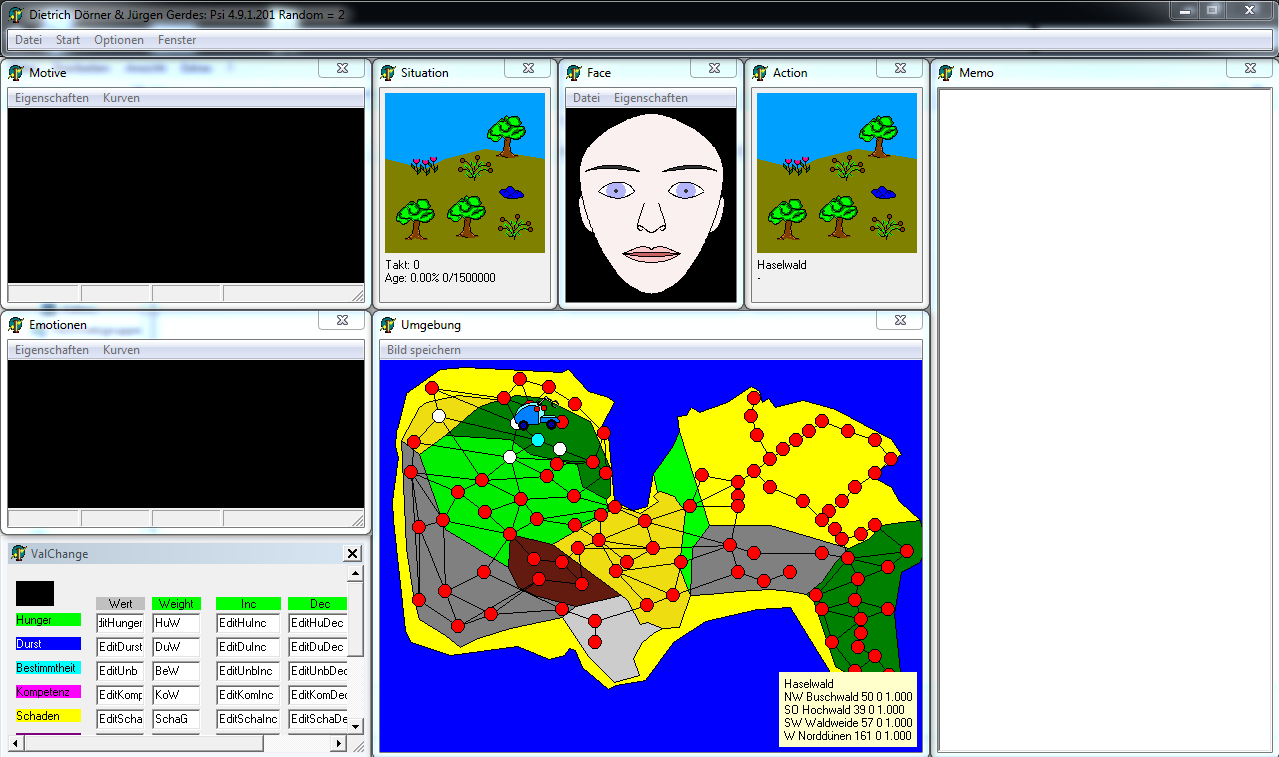
\includegraphics[width=10cm]{graphics/psi_screen1}
  \caption{Dörner's Pascal Psi Implementation}
  \label{psi_screen}
\end{figure}

The work on Dörner's team's implementation has not been continued, so Joscha Bach and his associates built new implementations of Psi.

From 2003 to 2009 they built an implementation in Java as a set of plugins for the Eclipse IDE called MicroPsi. It included a graphical editor and a 3D simulation-environment. 

    \section{MicroPsi 2}
Aiming at better understandability and to maintain platform independence, MicroPsi has been built ground up again in 2012 --- using more lightweight Python code. What is remarkable about the new implementation called MicroPsi 2 (in the following MicroPsi), is that the simulation is deployed as a web application and the graphical interface is completely rendered inside a web browser --- using state-of-the-art internet- and webapplication-technologies. It is based upon HTML as well as Javascript and the communication in between the browser and the simulation is managed via JSON remote procedure calls. Many GUI components of Twitter's Bootstrap library as well as the JavaScript graphics library PaperJS are used.~\cite{conf/agi/Bach12}

According to the concepts of the Psi Theory, MicroPsi simulates agents as neuro-symbolic spreading activation networks. Agents can be placed and researched in simulation environments or physically embodied as robots.~\cite{conf/agi/Bach12}
        
Even though there have been more complex simulation environments (e.g. 3D-worlds) for previous implementations of Psi-architectures, the relatively new version of MicroPsi has only two fairly simple ones: a 2D-Island and a map of the public transportation system of Berlin~(see figure~\ref{mp2_berlin}). Instead of building a new 3D-world, with this project we set out for something more experimental.

\begin{figure}[h]
  \centering
    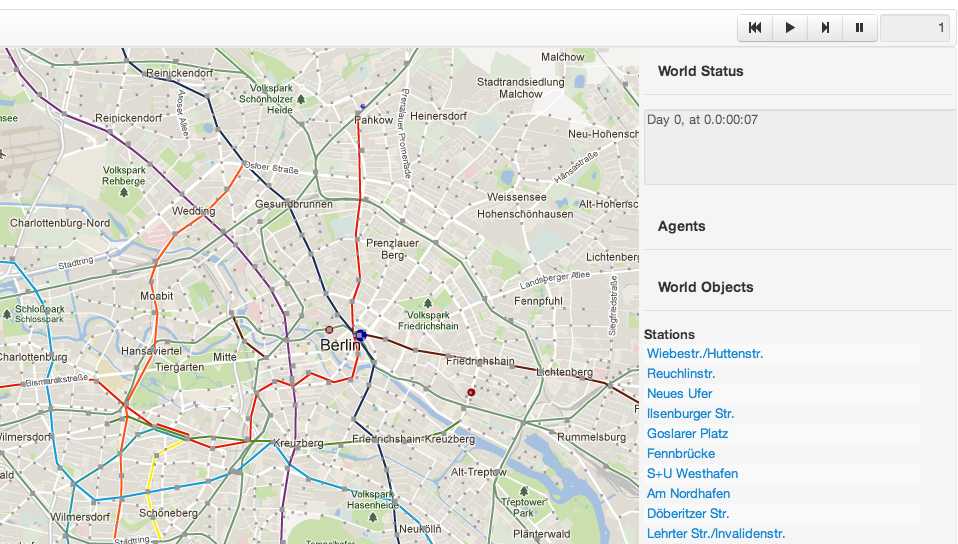
\includegraphics[width=10cm]{graphics/mp2_berlin}
  \caption{MicroPsi simulation environment Berlin}
  \label{mp2_berlin}
\end{figure}

        \subsection{Module Overview}
MicroPsi's modular structure is fairly easy to understand~(see figure ~\ref{micropsi2_modules}). At first, one can differentiate between the server component (or the web-interface) and the actual simulation code (called "core").

In a minimal setup MicroPsi runs three threads. One thread for the web server, one for the world simulation and one for every world-adapter (or agent). If more then one agent or more than one world are launched, they are instantiated as additional threads.

Furthermore, the core consists of a runtime component, a user and a configuration manager. The runtime works independently of the server and can also by deployed for command line interaction or other GUIs. It manages the simulations worlds as well as the agents (node net embodiments) and the world-adapters.~\cite{conf/agi/Bach12}
\\          
          
\begin{figure}[h]
  \centering
    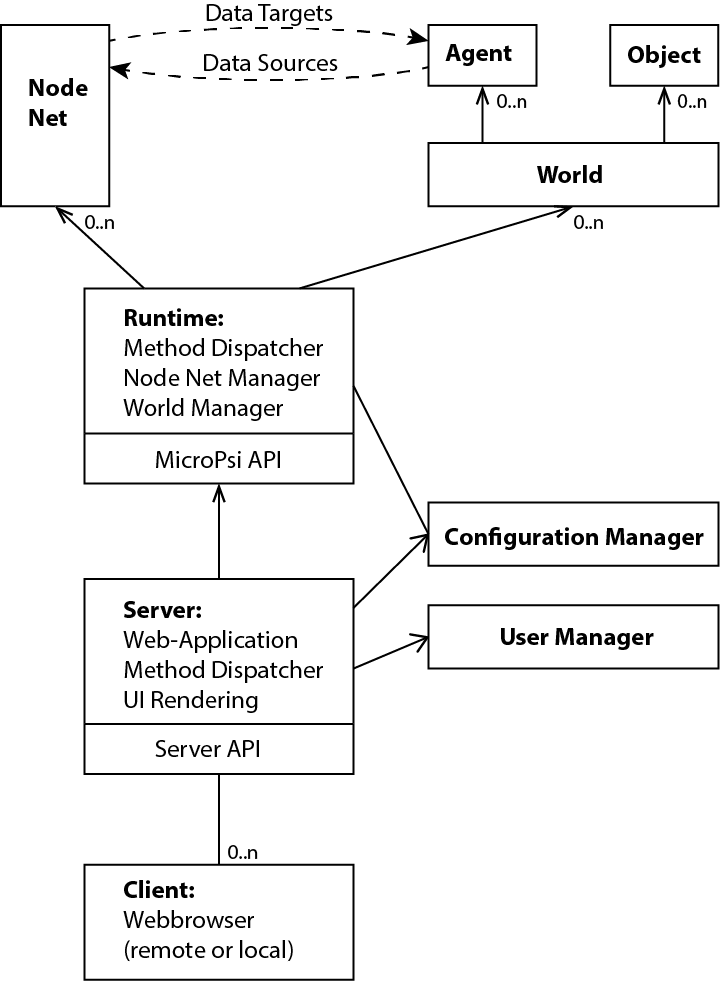
\includegraphics[width=10cm]{graphics/micropsi2_uml}
  \caption{The MicroPsi 2 architecture(taken from ~\cite{conf/agi/Bach12})}
  \label{micropsi2_modules}
\end{figure}

The following description is based on \cite{conf/agi/Bach12}, where the theoretical foundations can be found in more detail.

A graphical Editor is the primary interface.

MicroPsi is written in Python with a minimum of dependencies.

        \subsection{Module Server}
The Server module renders the GUI and deploys the agent simulation as a web application. It acts as a web server for remote or local access. Therefore simulations can be launched from anywhere without requiring any installation. It implements the lightweight Python web framework Bottle. The server communicates with its users through the server API. User sessions and access rights are managed by the user manager component. 
    
    Method Dispatcher
    UI Rendering
    User Manager / a user manager
    
A client for this application may be any computer with a reasonable up-to-date web browser - be it remote or local.
 
    
        \subsection{Module Runtime}
The server starts the runtime component, even though it may also work independently of the server. The runtime component communicates with the server through the MicroPsi API. It manages node nets and Worlds generates threads for each node net and World that has been started.

        \subsubsection{Node Nets}
A MicroPsi node net is defined as a set of states, a starting state, a network function," that determines how to advance to the next state" and a set of node types. "Data sources and data targets provide a connection to the environment; a data source represents a value that is determined by an environ- mental state, while the values of data targets can be changed to effect something in the environment."

"Each node is characterized by its identifier, its type, an optional set of pa- rameters (which can make the node stateful), a set of gates and a set of slots. Gates are outlets for activation, while slots are inlets."

"The types of slots and gates of a node are defined within the node type, next to ad- ditional functionality f ! performed by the node whenever it becomes active. In most cases, f ! is limited to transmitting activation within the node, from the standard slot ‘gen’ to the gates."

"Nodes can store additional parameters and change them in the course of the node function, which makes them state machines:"

"More generally, some nodes may contain arbitrary functions, such as the creation of new nodes and links, procedures for neural learning, planning modules etc. These functions take the form of a program in a native programming language (here, Py- thon), and hence, such nodes are also called native modules."



        \subsubsection{Worlds}
The simulations worlds are the environments in which we can study our agent's behaviour. Worlds need to provide a world adapter --- the interface in between a node net and the simulation. Data sources and data targets have to be defined carefully, to get a functional and meaningful experiment going. Node nets and environments may be updated asynchronously.~\cite{conf/agi/Bach12}

The kind of data the world adapter interfaces, is not specified any further, which gives developers the opportunity to experiment with classic simulation worlds as well as exotic applications (eg. stock data). At the time of the original development of the framework, the priorized application was building a framework for knowledge representation.~\cite{conf/agi/Bach12}

"Within the MicroPsi framework, agents may be embedded into an environment. The environment must provide a world adapter for each MicroPsi agent. The world adapter offers data sources, from which the agent’s node net may read environmental information, and data targets, which allow the agent to effect changes in the world. Since the environment only has write access to data sources, and read access to data targets, node net and environment may be updated asynchronously.
The world adapter may interface a local multi-agent simulation, a robotic body, a computer game client or simulation server, dynamically updated stock data, etc. Here, we give a simple simulation world as an example."

"Objects have a position (for instance ), a set of object states and an object function, that determines how the position and states of the object change from one state to the next, based on the previous state, the states and positions of oth- er objects and the terrain."

"Agents are objects in the world like any other, but each agent object corresponds to
a world adapter, which links it to a node net. Think of the agent object as the body of
the MicroPsi agent, and the object states as its physiological states. The object func-
tion of the agent f advances these physiological states, the position of the agent
and the inputs to the node net.
In each simulation step, the world function calls all object functions, and takes care
of the creation of new objects and the removal of obsolete ones."

        \paragraph{Agents}    
        
MicroPsi defines agents as node nets or, to be more specific, hierarchical spreading activation networks. They are an "abstraction of the information processing provided by brains"~\cite{conf/agi/Bach12}. The assigned world-adapter provides data sources and data targets to manage the communication in between the node net and the simulation environment. They represent the agent's sensory input and motoric output. Sophisticated interconnection of those enables interaction with the environment.~\cite{conf/agi/Bach12}
As node nets share the relevant characteristics with neural node nets, they may enable neural learning paradigms. To store information they can form semantic networks. Furthermore, nodes may contain state machines and other operations, which make it possible to build modularized architectures.

        \paragraph{Objects}
Objects can be things like lightsources.
 
    Method Dispatcher
    Node Net Manager
        Node Net / a set of node nets,
    World Manager
        World / a set of simulation worlds,
            Agent
            Object
    (MicroPsi API)
    



(Data Targets / Data Sources)







\begin{figure}[h]
  \centering
    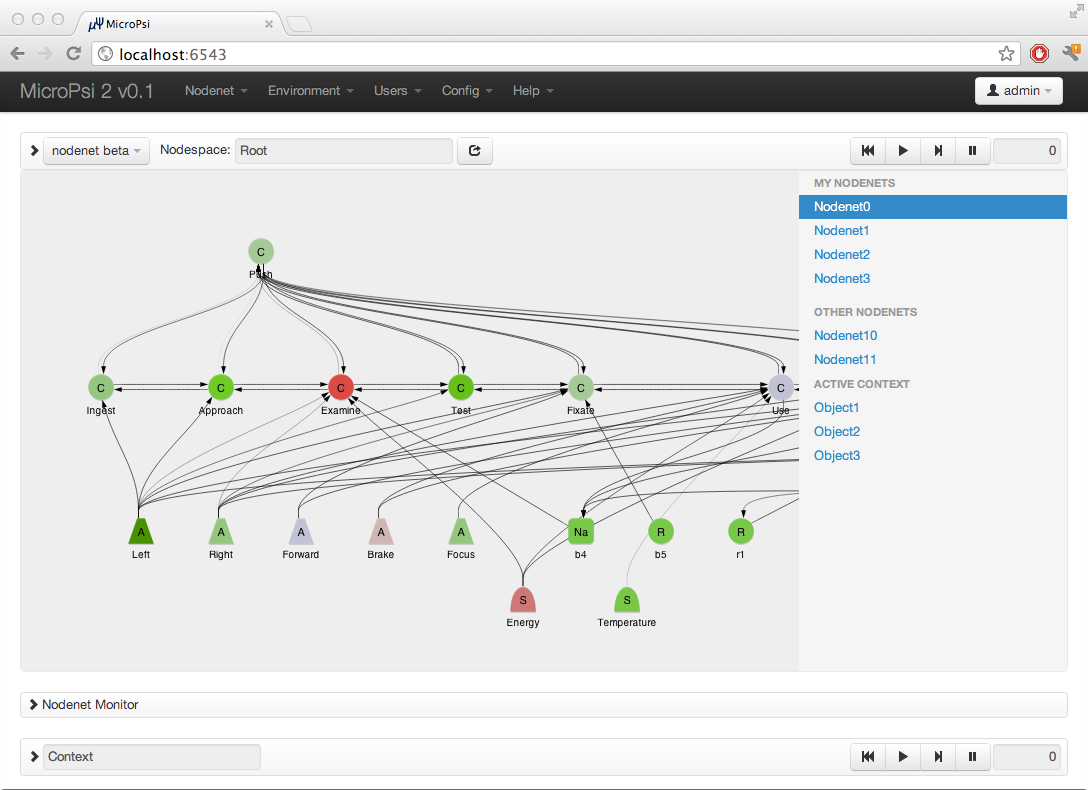
\includegraphics[width=10cm]{graphics/micropsi2_nodenet}
  \caption{A MicroPsi 2 nodenet. (taken from ~\cite{conf/agi/Bach12})}
  \label{micropsi2_nodenet}
\end{figure}